\section{Conduction}%
\label{sec:conduction}
\begin{wrapfigure}{r}{0.6\textwidth}
		\centering
		\includegraphics[width=1.0\linewidth]{./build/emissionconstruction.pdf}
		\caption{Sketch of the setup to check if the laser produce induce or
		spontaneous emission. \cite{anleitung}}
		\label{fig:aufbau}
\end{wrapfigure}
For further observation with a laser, you have to attitude it first. 
First thing to do is to calibrate the current to achieve a population inversion. 
For making the laser light visible the laser is pointed to a buisnesscardholder
which is filmed by a ccd sensor.
To achieve the minimal current to laser by induce emission, alternately the head
knob and side knob position is optimized.
Every time stimulated emission is produce, current is reducing a
little bit. 
The last visible induce emission is an estimation of the minimal laser current.
A note for stimulated emission is the light cone from induced emission, is
much brighter and more homogeneous than by spontaneous Emission.
One example for induce \ref{fig:induce} and spontaneous \ref{fig:spontanious} light cone is shown in picture \ref{fig:emission}.
\begin{figure}[h]
		\centering
		\begin{subfigure}[b]{0.45\textwidth}
				\begin{center}
						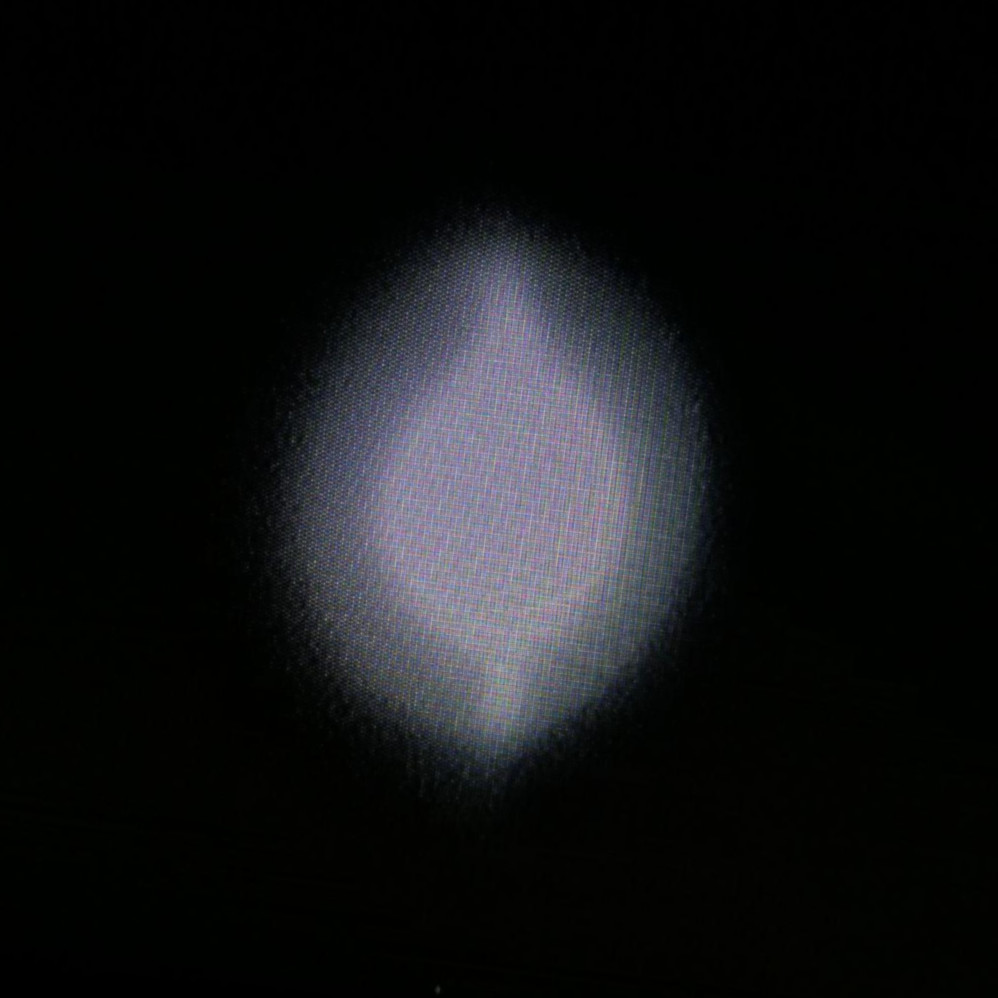
\includegraphics[width=0.7\linewidth]{./content/pictures/below_threshold.jpg}
						\caption{spontaneous emission}
				\label{fig:spontanious}
				\end{center}
		\end{subfigure}
		\begin{subfigure}[b]{0.45\textwidth}
				\begin{center}
						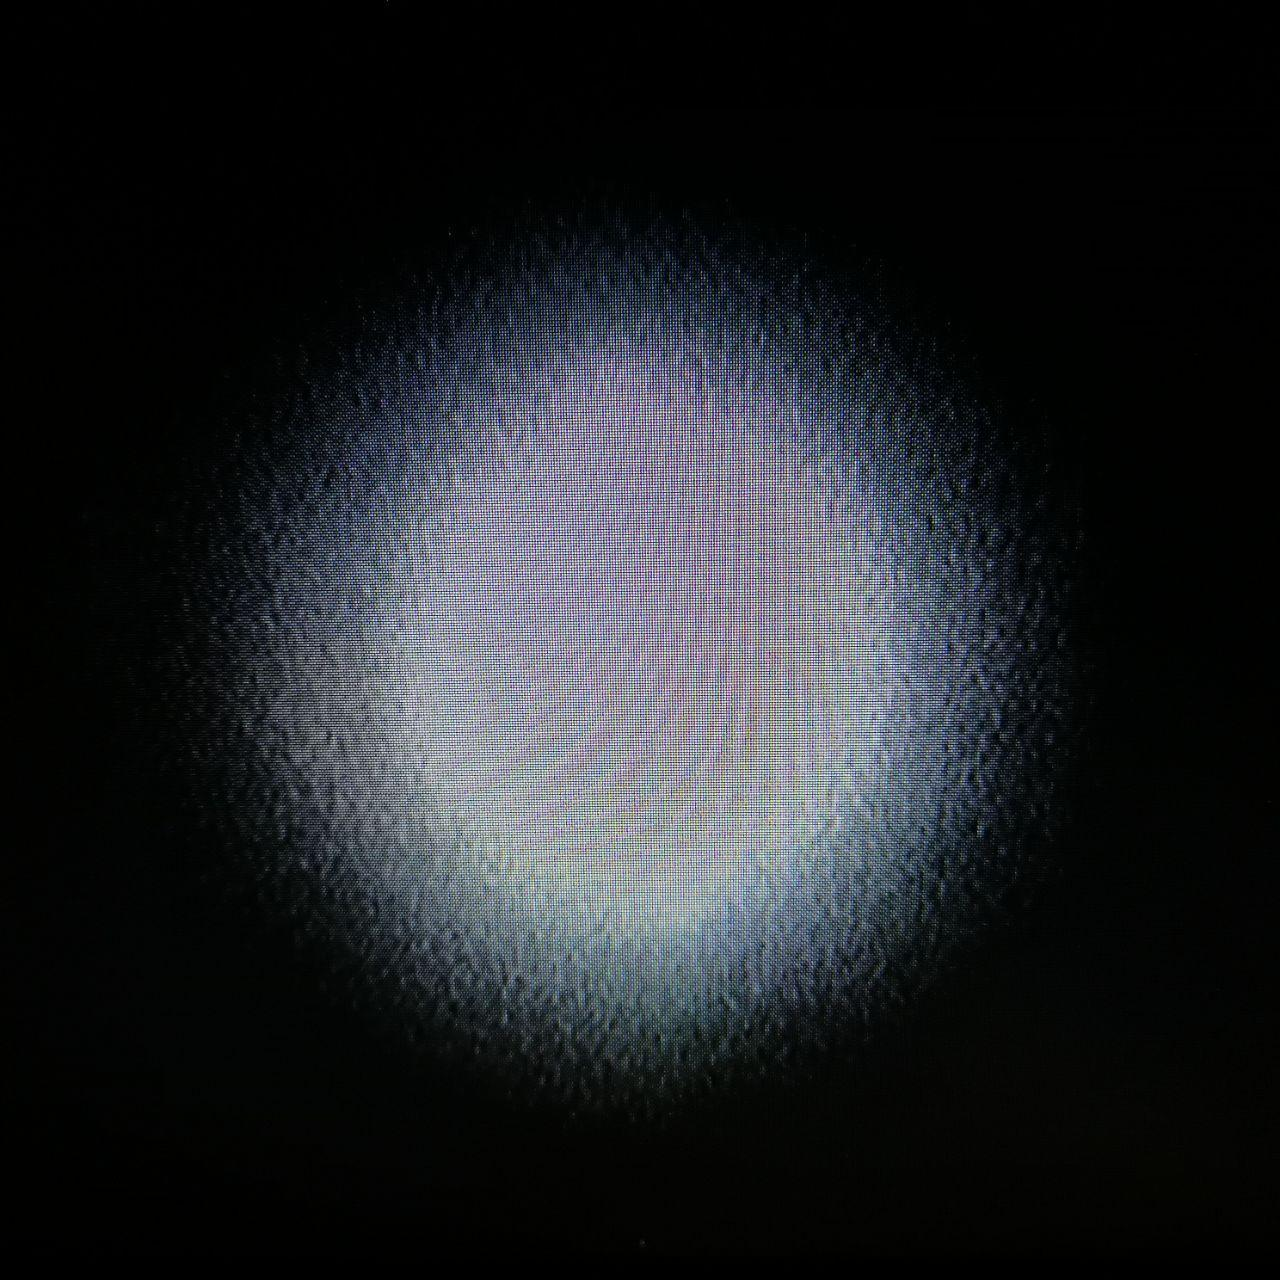
\includegraphics[width=0.7\linewidth]{./content/pictures/above_threshold.jpg}
						\caption{induce emission}
						\label{fig:induce}
				\end{center}
		\end{subfigure}
		\caption{Light emission of a diode laser visible on a fluorescence
		paper observed by a ccd camera.}
		\label{fig:emission}
\end{figure}
The measured current for the minimal threshold is \SI{30}{\milli\ampere}.
By moving both knobs over full range, no flashes can be generated.

\subsection{Fluorescence Rubidium}%
\label{sub:anregen_rubidium}

To stimulated the rubidium gas beam angle has to pass the chamber, that no
light is sprinkled at the border of the chamber. 
Figure \ref{fig:hole_emission} shows how the measuring instrument have to be
arrange for measure the light intensity.
\begin{figure}[h]
		\centering
		\includegraphics[width=0.8\linewidth]{build/rubidiumemission.pdf}
		\caption{Sketch of a setup to measure the spectrum of Rubidium and
		aligning the laser on right frequency.\cite{anleitung}}
		\label{fig:hole_emission}
\end{figure}
A photo diode is placed behind the Rb-cell to measure the laser light which
passing the cell.
The voltage of the photo diode is increased and shown on an oscilloscope. 
The side knob have to be calibrate to attain the right frequency for stimulating
the gas. 
A grating is put in the beam for reducing the contrast so that the beam angle
can be seen with help of a ccd camera. 
If in the camera a small beam is visible, searched frequency is be found. 
The middle beam of side knob variation should be chosen because it had the
strongest gain.
An example for fluorescence rubidium is shown in figure \ref{fig:ionized}.
\begin{figure}[h]
		\centering
		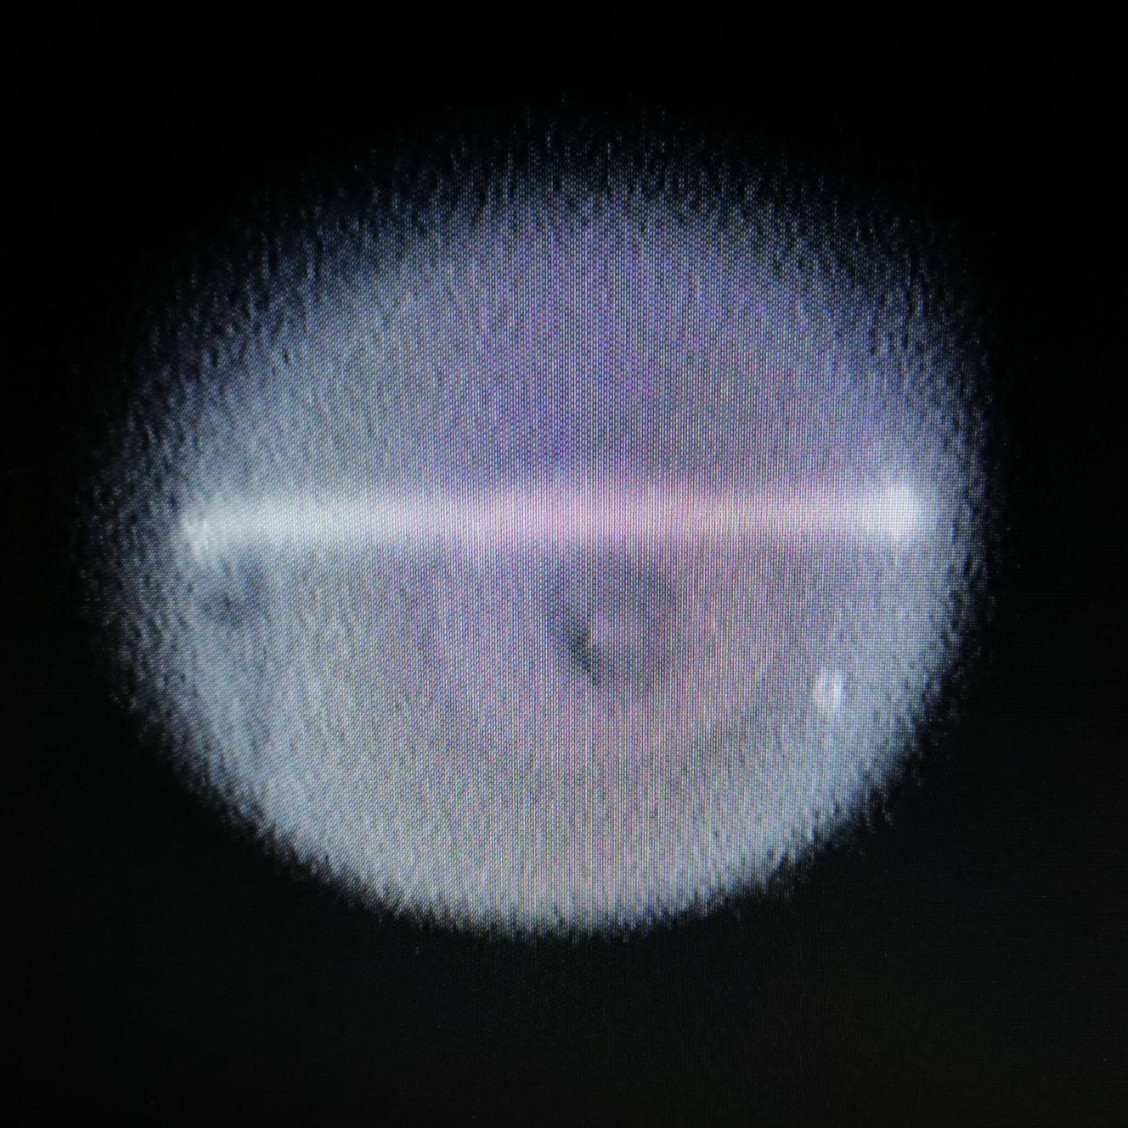
\includegraphics[width=0.4\linewidth]{./content/pictures/fluorescence.jpg}
		\caption{Fluorescence of rubidium filmed by ccd camera with 
				\SI{69.9}{\milli\ampere} laser current.}
		\label{fig:ionized}
\end{figure}
After the Rubidium is fluorescence aim is to measure the absorption spectrum. 

\subsection{Absorbtion spectrum}%
\label{sub:absorbtion_spectrum}

An absorption spectrum is dependence from the frequency. 
To achieve a variation in frequency a piezo element is used. 
The piezo element is on the diffraction grating to variated the length of the
external cavity. 
Variation of cavity length causes shifts in laser frequency. 
Piezo element is powered by a ramp generator which causes linear shifts in
cavity length in a defined time period.
When photon current is measured by a sensor dependence between energy levels can
be plotted.
\begin{figure}[h]
		\centering
		\begin{subfigure}[b]{0.49\textwidth}
				\begin{center}
				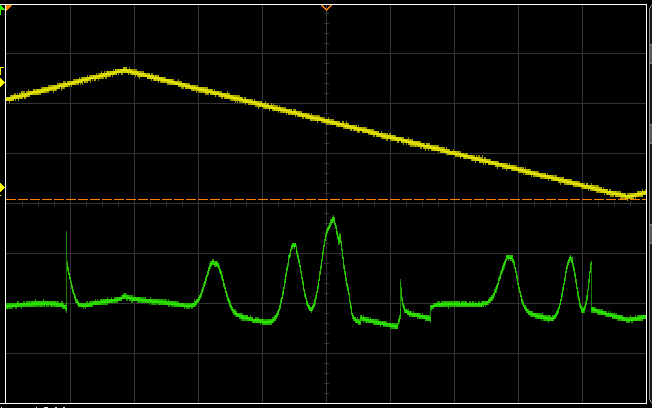
\includegraphics[width=1.0\linewidth]{./content/pictures/scope_136.png}
						\caption{mode hopping}
				\label{fig:piezotest}
				\end{center}
		\end{subfigure}
		\begin{subfigure}[b]{0.49\textwidth}
				\begin{center}
						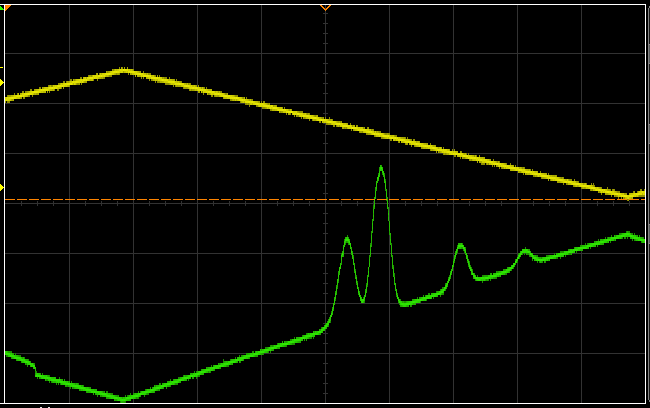
\includegraphics[width=1.0\linewidth]{./content/pictures/scope_138.png}
						\caption{triangle background}
						\label{fig:rectangular}
				\end{center}
		\end{subfigure}
		\caption{Absorption spectrum with undesired side effects.}
		\label{fig:}
\end{figure}
In figure \ref{fig:piezotest} the yellow line shows the voltage at the Piezo
element which causes frequency variation proportional to voltage.
The green line is photo stream. 
Hopes in the photon stream are horizontal modes caused by the Piezo element.
They are of no further interest.
Mode hopping can be reduced by modulation with the piezo voltage. 
The response is the figure \ref{fig:rectangular}.
The characteristic spectrum of a rubidium crystal is visible which the
absorption lines. 
In general the green line should be mirrored on the x-axis because resonance
reduce the Energy on the photon stream. 
For achieving a flat spectrum which is not depended of the piezo voltage some
modification are necessary.

\subsection{Modulated spectrum}%
\label{sub:modulated_spectrum}

For modulation of the inital laser beam and this which passes the medium, beam
will be splited in two parts. 
A semipermeable mirror will be set in the beam path in front of the medium. 
Light which reflected before the medium will be measured by a second Photomultiplier.
Now beam modulation with a part which not passes and a part which passes the
medium can be done. 
The absorption spectrum without piezo movement effect is shown in figure
\ref{fig:modulation}.
\begin{figure}[h]
		\centering
		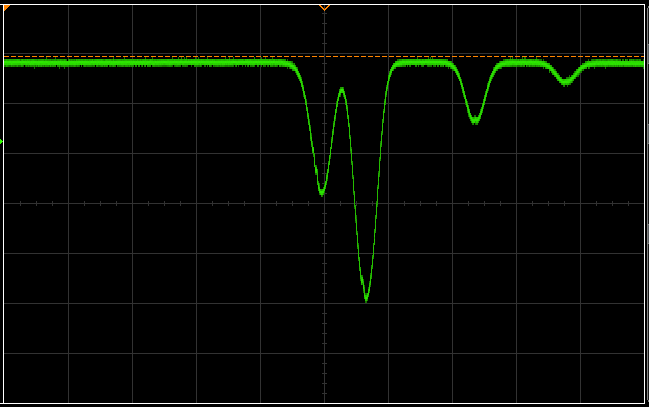
\includegraphics[width=0.8\linewidth]{./content/pictures/scope_140.png}
		\caption{Absorption spectrum of rubidium.}
		\label{fig:modulation}
\end{figure}
There are the different energy levels (85\sfrac{a}{b}, 87\sfrac{a}{b}) are
visible.
Know the laser is aligned and ready for further experiments.
